\chapter{ขั้นตอนวิธี}\label{ch:methodology}

\section{ภาพรวมของขั้นตอนวิธี}\label{sec:ch4_methodology_overview}
\paragraph{}
กระบวนการดำเนินงานของโครงการวิจัยนี้เป็นไปตามกรอบการทำงาน KGs-Augmented Testsuite Generator Framework ซึ่งถูกออกแบบมาเพื่อเปลี่ยนรายงานอุบัติเหตุที่เป็นข้อความ (Unstructured Text) ให้กลายเป็นชุดทดสอบ (Test Suite) ที่มีโครงสร้างและมุ่งเน้นการค้นหา Edge-Case อย่างมีประสิทธิภาพ หัวใจสำคัญของขั้นตอนวิธีคือการทำงานร่วมกันของเทคโนโลยีสามส่วนหลัก ได้แก่ Schema-guided LLM, Knowledge Graph (KG) และ Inference Engine ที่ใช้กฎของ Operational Design Domain (ODD) โดยเฉพาะอย่างยิ่งการใช้เทคนิค Query Rotation ผ่านกลุ่มของ ODD ที่เรียกว่า ODD Modular เพื่อให้การค้นหามีความครอบคลุมและเป็นระบบ ผลลัพธ์สุดท้ายของกระบวนการนี้ไม่ใช่ไฟล์สถานการณ์จำลองที่สมบูรณ์ แต่เป็นชุดของ พารามิเตอร์ (Parameters) ที่พร้อมสำหรับนำไปใช้กับ Scenario Template ที่มีอยู่แล้วในขั้นตอนการทดสอบจริง โดยกระบวนการทั้งหมดสามารถสรุปเป็นอัลกอริทึมได้ดังแสดงใน Algorithm~\ref{alg:main_framework}

\begin{algorithm}[H]
\caption{KGs-Augmented Testsuite Generation Framework with Modular Query}
\label{alg:main_framework}
\begin{algorithmic}[1]
\State \textbf{Input:} \textit{AccidentReports} (ชุดรายงานอุบัติเหตุ), \textit{ODDModularGroups} (กลุ่มของกฎ ODD)
\State \textbf{Output:} \textit{GeneratedParameters} (ชุดของพารามิเตอร์สำหรับ Scenario Templates)

\Procedure{GenerateTestsuite}{\textit{AccidentReports, ODDModularGroups}}
    \State \textit{StructuredDataList} $\gets$ []
    \State \textit{KnowledgeGraph} $\gets$ InitializeEmptyGraph()

    \Comment{\textbf{ขั้นที่ 1: การสกัดข้อมูลอุบัติเหตุ (Data Extraction)}}
    \ForAll{\textit{report} \textbf{in} \textit{AccidentReports}}
        \State \textit{structuredData} $\gets$ \Call{ExtractStructuredData}{\textit{report}}
        \State \textit{StructuredDataList}.add(\textit{structuredData})
    \EndFor

    \Comment{\textbf{ขั้นที่ 2: การสร้าง Knowledge Graph (KG Modeling)}}
    \ForAll{\textit{data} \textbf{in} \textit{StructuredDataList}}
        \State \Call{BuildKnowledgeGraph}{\textit{KnowledgeGraph, data}}
    \EndFor

    \Comment{\textbf{ขั้นที่ 3: การค้นหา Edge-Case ด้วย Query Rotation}}
    \State \textit{AllEdgeCaseEvents} $\gets$ []
    \ForAll{\textit{modularGroup} \textbf{in} \textit{ODDModularGroups}}
        \State \textit{foundEvents} $\gets$ \Call{QueryCasesByModular}{\textit{KnowledgeGraph, modularGroup}}
        \State \textit{AllEdgeCaseEvents}.addRange(\textit{foundEvents})
    \EndFor

    \Comment{\textbf{ขั้นที่ 4: การสร้างชุดพารามิเตอร์จาก Edge-Case}}
    \State \textit{GeneratedParameters} $\gets$ []
    \ForAll{\textit{event} \textbf{in} \textit{AllEdgeCaseEvents}}
        \State \textit{params} $\gets$ \Call{GenerateParametersFromEvent}{\textit{event}}
        \State \textit{GeneratedParameters}.add(\textit{params})
    \EndFor

    \State \textbf{return} \textit{GeneratedParameters}
\EndProcedure
\end{algorithmic}
\end{algorithm}

\section{ขั้นตอนการดำเนินงานโดยละเอียด}\label{sec:ch4_methodology}

\subsection{ขั้นที่ 1: การสกัดข้อมูลอุบัติเหตุที่มีโครงสร้าง (Structured Data Extraction)}\label{subsec:ch4_data_extraction}
\paragraph{}
ขั้นตอนแรกคือการแปลงรายงานอุบัติเหตุที่ไม่มีโครงสร้างให้เป็นข้อมูลที่มีโครงสร้างที่ชัดเจน โดยใช้โมเดลภาษาขนาดใหญ่ (LLM) ที่ถูกควบคุมทิศทางด้วย Schema ที่ออกแบบไว้ล่วงหน้า เพื่อให้มั่นใจได้ว่าข้อมูลสำคัญทั้งหมดจะถูกสกัดออกมาอย่างครบถ้วนและสม่ำเสมอ กระบวนการนี้สรุปได้ดัง Function \Call{ExtractStructuredData}{}

\begin{algorithmic}[1]
\Function{ExtractStructuredData}{\textit{report}}
    \Comment{ใช้เทคนิค Multi-Step Prompting เพื่อความแม่นยำ}
    \State \textit{worldData} $\gets$ LLM.extract(\textit{report, worldSchema})
    \State \textit{actorData} $\gets$ LLM.extract(\textit{report, actorSchema})
    \State \textit{sequenceData} $\gets$ LLM.extract(\textit{report, sequenceSchema})
    \State \textbf{return} \{\textit{world: worldData, actors: actorData, sequence: sequenceData}\}
\EndFunction
\end{algorithmic}

\paragraph{}
ผลลัพธ์จากขั้นตอนนี้คือชุดข้อมูลที่มีโครงสร้าง (เช่น ในรูปแบบ JSON) ซึ่งแยกองค์ประกอบของอุบัติเหตุออกเป็น 3 ส่วนหลัก ได้แก่ \textbf{World}, \textbf{Actors}, และ \textbf{Sequence} ดังแสดงตัวอย่างในรูปที่~\ref{fig:ch4_extracted_data}

\begin{figure}[htbp]
    \centering
    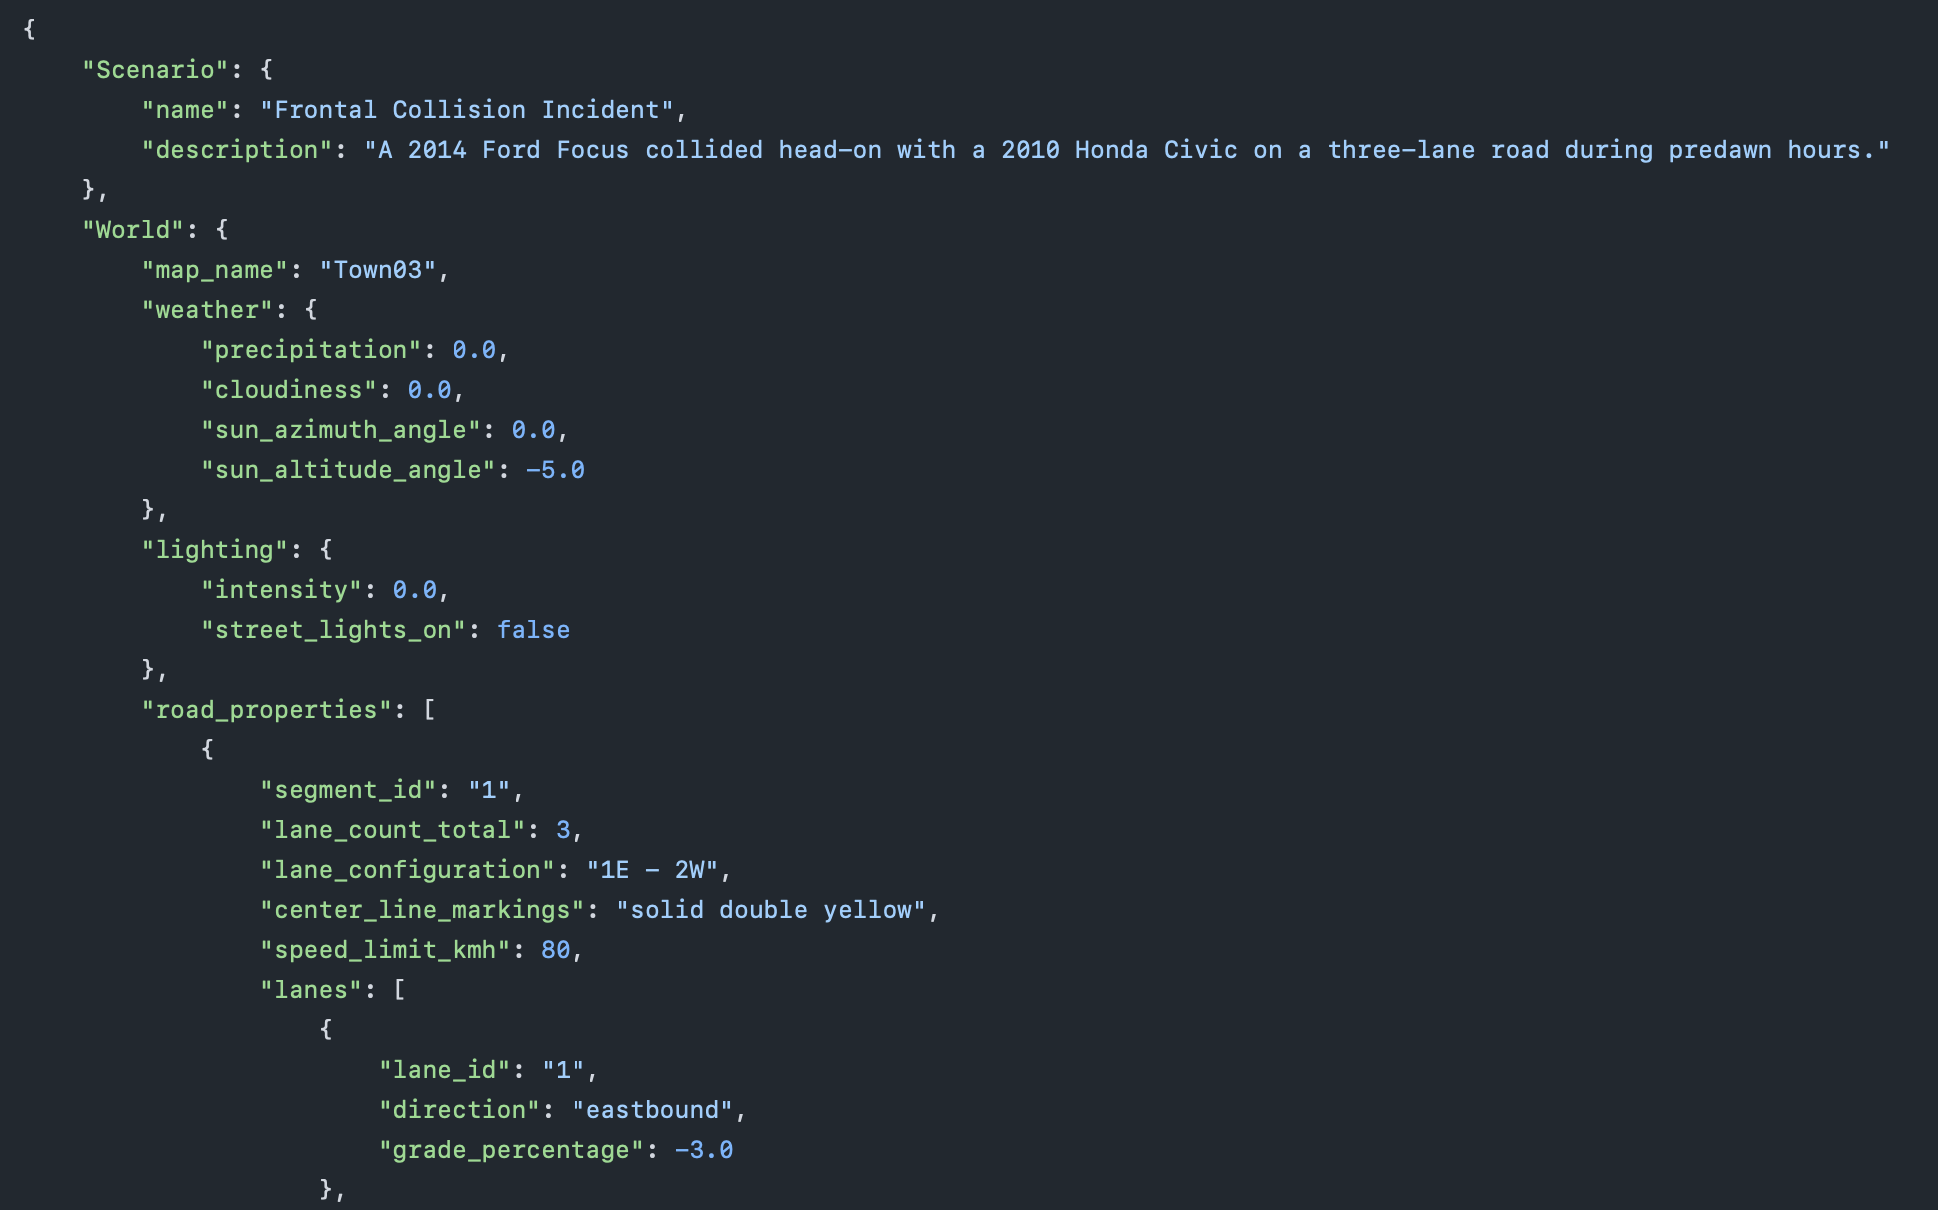
\includegraphics[width=0.8\textwidth]{images/kg-extracted-data-example}
    \caption{ตัวอย่างโครงสร้างข้อมูลที่ได้จากการสกัดรายงานอุบัติเหตุ C00013 โดย Schema-guided LLM}
    \label{fig:ch4_extracted_data}
\end{figure}

\subsection{ขั้นที่ 2: การสร้าง Knowledge Graph (KG Modeling)}\label{subsec:ch4_kg_modeling}

\paragraph{}
ข้อมูลที่มีโครงสร้างจากขั้นตอนที่ 1 จะถูกนำมาสร้างเป็น Knowledge Graph (KG) ซึ่งทำหน้าที่เป็น Semantic Backbone ของข้อมูลอุบัติเหตุทั้งหมด โดยการแปลงข้อมูลแต่ละส่วนให้เป็นโหนด (Nodes) และความสัมพันธ์ (Relationships) ดังกระบวนการใน Function \Call{BuildKnowledgeGraph}{}

\begin{algorithmic}[1]
\Function{BuildKnowledgeGraph}{\textit{graph, data}}
    \Comment{แปลงข้อมูล JSON เป็น Nodes และ Relationships}
    \State Create Nodes for actors, events, environment from \textit{data}
    \State Create Relationships (e.g., :CAUSED\_BY, :OCCURRED\_IN) between nodes
    \State Add nodes and relationships to \textit{graph}
\EndFunction
\end{algorithmic}

\paragraph{}
ผลลัพธ์ที่ได้คือ Knowledge Graph ที่สามารถแสดงความเชื่อมโยงที่ซับซ้อนของปัจจัยต่างๆ ในอุบัติเหตุได้อย่างชัดเจน ดังตัวอย่างในรูปที่~\ref{fig:ch4_kg_model}

\begin{figure}[htbp]
    \centering
    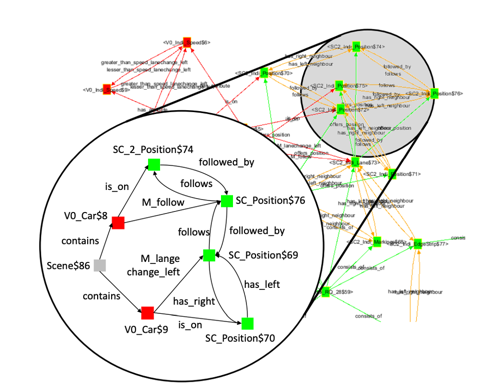
\includegraphics[width=1\textwidth]{images/kg-model-example}
    \caption{ตัวอย่างส่วนหนึ่งของ Knowledge Graph ที่แสดงความสัมพันธ์ของเอนทิตีในอุบัติเหตุ C00013}
    \label{fig:ch4_kg_model}
\end{figure}


\subsection{ขั้นที่ 3: การบูรณาการ ODD และการค้นหา Edge-Case ด้วย Query Rotation}\label{subsec:ch4_odd_integration}

\paragraph{}
ขั้นตอนนี้คือหัวใจสำคัญของกรอบการทำงานซึ่งใช้เทคนิค Query Rotationเพื่อค้นหาสถานการณ์ที่ท้าทายระบบ (Edge-Case) อย่างเป็นระบบ โดยใช้ ODD Modular ซึ่งเป็นกลุ่มของเงื่อนไข ODD ที่ถูกกำหนดไว้ล่วงหน้าเพื่อแทนสถานการณ์อันตรายประเภทต่างๆ (เช่น กลุ่ม "การชนท้าย") จากนั้น อัลกอริทึมจะวนลูปเพื่อสืบค้น (Query) เหตุการณ์ใน Knowledge Graph ทีละ Modular ทำให้มั่นใจได้ว่ามีการค้นหาที่ครอบคลุมในทุกมิติของความเสี่ยง กระบวนการนี้สรุปได้ดัง Function \Call{QueryCasesByModular}{}

\begin{algorithmic}[1]
\Function{QueryCasesByModular}{\textit{graph, modularGroup}}
    \State \textit{InferenceEngine} $\gets$ InitializeEngine(\textit{graph})
    \State \textit{rules} $\gets$ modularGroup.getRules()
    \State \textit{MatchingEvents} $\gets$ \textit{InferenceEngine}.query(\textit{rules})
    \Comment{เช่น ค้นหา Event ที่ตรงตามเงื่อนไขของ Modular ที่กำหนด}
    \State \textbf{return} \textit{MatchingEvents}
\EndFunction
\end{algorithmic}

\paragraph{}
เมื่อระบบทำงานกับ Modular "การฝ่าฝืนสัญญาณจราจร" Inference Engine จะค้นหาเหตุการณ์ทั้งหมดใน KG ที่เข้าข่ายเงื่อนไขนี้ เช่น `Event\_RunRedLight` ในกรณี C00013 และระบุว่าเป็น Edge-Case ที่ตรงกับ Modular ดังกล่าว ดังแสดงในรูปที่~\ref{fig:ch4_kg_inference}

\begin{figure}[htbp]
    \centering
    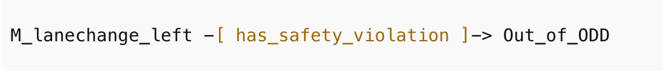
\includegraphics[width=1\textwidth]{images/kg-inference-example}
    \caption{Knowledge Graph หลังจากผ่าน Inference Engine โดยมีการสร้างความสัมพันธ์ใหม่ (เส้นสีแดง) เพื่อระบุว่าเหตุการณ์ฝ่าไฟแดงเป็น Edge-Case ที่ตรงกับ ODD Modular "การฝ่าฝืนสัญญาณจราจร"}
    \label{fig:ch4_kg_inference}
\end{figure}

\subsection{ขั้นที่ 4: การสร้างชุดพารามิเตอร์สำหรับ Scenario Template}\label{subsec:ch4_scenario_generation}

\paragraph{}
ในขั้นตอนสุดท้าย กรอบการทำงานไม่ได้สร้างไฟล์ `.xosc` ออกมาโดยตรง แต่จะดำเนินการในลักษณะที่ยืดหยุ่นกว่า คือการสร้าง ชุดพารามิเตอร์ (Parameter Set) จากข้อมูล Edge-Case ที่ค้นพบในขั้นตอนที่ 3 พารามิเตอร์เหล่านี้คือค่าตัวแปรที่สำคัญของสถานการณ์ เช่น ความเร็วเริ่มต้นของรถ, ตำแหน่ง, ประเภทของยานพาหนะ, สภาพถนน เป็นต้น

\begin{algorithmic}[1]
\Function{GenerateParametersFromEvent}{\textit{eventData}}
    \Comment{Map ข้อมูลจาก KG node ไปเป็นโครงสร้าง Key-Value}
    \State \textit{params} $\gets$ new Dictionary()
    \State \textit{params}["initial\_speed\_v1"] $\gets$ \textit{eventData}.getVehicle(1).speed
    \State \textit{params}["road\_friction"] $\gets$ \textit{eventData}.getEnvironment().surfaceFriction
    \State \textit{params}["maneuver\_actor"] $\gets$ \textit{eventData}.getActor().id
    \State \textbf{return} \textit{params}
\EndFunction
\end{algorithmic}

\paragraph{}
ชุดพารามิเตอร์ที่ได้นี้จะถูกจัดเก็บไว้ และในขั้นตอนการทดสอบจริง ผู้ใช้จะเลือก Scenario Template (เช่น Template สำหรับสถานการณ์ Cut-in, Template สำหรับสถานการณ์ Unsignalized Left-Turn) ซึ่งเป็นไฟล์ `.xosc` ที่มีโครงสร้างทั่วไปและมีช่องว่างสำหรับรับค่าพารามิเตอร์ จากนั้นจึงนำชุดพารามิเตอร์ที่ Framework สร้างขึ้นไปเติมใน Template เพื่อสร้างเป็น Test Case ที่สมบูรณ์และพร้อมใช้งานต่อไป วิธีการนี้ช่วยแยกส่วนระหว่าง "ข้อมูล" (Parameters) และ "ตรรกะของสถานการณ์" (Template) ออกจากกัน ทำให้สามารถสร้าง Test Case ที่หลากหลายได้อย่างมีประสิทธิภาพและนำกลับมาใช้ซ้ำได้ง่าย
\section{ขั้นตอนการประเมินผล: Scenario Completeness Score}\label{sec:ch4_evaluation_method}
\paragraph{}
เพื่อให้สามารถประเมินคุณภาพของสถานการณ์จำลองที่สร้างขึ้นได้อย่างเป็นรูปธรรมและมีมาตรฐาน กรอบการทำงานนี้ได้กำหนดวิธีการประเมินเชิงปริมาณที่เรียกว่า \textbf{Scenario Completeness Score} (หรือ R-score) ขึ้นมา โดยมีวัตถุประสงค์เพื่อวัดคุณภาพเชิงฟังก์ชัน (Functional Quality) ของ Knowledge Graph ที่ได้จากระบบ เปรียบเทียบกับกราฟต้นฉบับ (Ground Truth) ที่สร้างขึ้นจากรายงานอุบัติเหตุจริง

\paragraph{}
หัวใจสำคัญของการประเมินคือการให้น้ำหนัก (Weighting) กับความสัมพันธ์ (Edges/Relationships) แต่ละประเภทตามความสำคัญที่มีต่อความสมจริงของสถานการณ์ (Scenario Fidelity) โดยคำนวณจากสูตรดังสมการที่~\ref{eq:completeness_score}

\begin{equation}
    \text{Score}_{\text{Weighted}} = \frac{\sum_{\text{Common Edges}} W_i}{\sum_{\text{All Edges in Both Graphs}} W_i}
    \label{eq:completeness_score}
\end{equation}

\paragraph{}
โดยที่:
\begin{itemize}
    \item \textbf{ตัวเศษ ($\sum_{\text{Common Edges}} W_i$):} คือผลรวมของค่าน้ำหนัก ($W_i$) ของความสัมพันธ์ทั้งหมดที่ปรากฏ \textbf{ร่วมกัน} ทั้งในกราฟต้นฉบับและกราฟที่ระบบสร้างขึ้น ซึ่งสะท้อนถึงองค์ประกอบของสถานการณ์ที่ระบบสามารถสร้างได้อย่างถูกต้อง
    \item \textbf{ตัวส่วน ($\sum_{\text{All Edges in Both Graphs}} W_i$):} คือผลรวมของค่าน้ำหนัก ($W_i$) ของความสัมพันธ์ทั้งหมดที่ไม่ซ้ำกันที่ปรากฏในกราฟใดกราฟหนึ่งหรือทั้งสองกราฟรวมกัน ซึ่งสะท้อนถึงข้อมูลที่เป็นไปได้ทั้งหมดของสถานการณ์
\end{itemize}

\paragraph{}
ค่าน้ำหนัก ($W_i$) ถูกกำหนดขึ้นโดยแบ่งตามประเภทและความสำคัญของความสัมพันธ์ ดังแสดงในตารางที่~\ref{tab:relationship_weights}

\begin{table}[htbp]
    \centering
    \caption{ค่าน้ำหนักของความสัมพันธ์ประเภทต่างๆ ตามความสำคัญต่อความสมจริงของสถานการณ์}
    \label{tab:relationship_weights}
    \begin{tabular}{|l|c|p{7cm}|}
        \hline
        \rowcolor{gray!20} \textbf{Relationship Type} & \textbf{Weight ($W_i$)} & \textbf{Importance to Scenario Fidelity} \\
        \hline
        Temporal/Causal & 3 & จำเป็นอย่างยิ่งต่อการกำหนดลำดับเหตุการณ์และความเป็นเหตุเป็นผลของอุบัติเหตุ \\
        (เช่น followed\_by, M\_follow) & & \\
        \hline
        Positional/Topological & 2 & จำเป็นต่อการกำหนดบริบทเชิงพื้นที่และขอบเขตของ ODD ที่แม่นยำ \\
        (เช่น is\_on, adjacent\_left) & & \\
        \hline
        Proximity/Trigger & 1 & จำเป็นต่อการกำหนดเงื่อนไขเริ่มต้น (Start Trigger) ของเหตุการณ์วิกฤต \\
        (เช่น near\_coll, very\_near) & & \\
        \hline
    \end{tabular}
\end{table}

\paragraph{}
ค่าคะแนนที่ได้จะมีค่าอยู่ระหว่าง 0 ถึง 1 โดยคะแนนที่เข้าใกล้ 1 หมายถึงกราฟที่ระบบสร้างขึ้นมีความสมบูรณ์และความสมจริงสูง สามารถจำลององค์ประกอบเชิงฟังก์ชันที่สำคัญของอุบัติเหตุต้นฉบับได้อย่างครบถ้วน

\section{ข้อจำกัดของการศึกษา}\label{sec:ch4_limitations}
\paragraph{}

การวิจัยนี้มุ่งเน้นการพัฒนากรอบการทำงานที่เป็นแนวคิดใหม่ในการสร้างชุดทดสอบ แต่ก็มีข้อจำกัดหลายประการที่ต้องนำมาพิจารณา ซึ่งส่วนใหญ่เกี่ยวข้องกับคุณภาพของข้อมูลนำเข้า ความจำกัดของเทคโนโลยีที่ใช้ และขอบเขตการดำเนินงานที่ถูกกำหนดไว้ล่วงหน้า ดังนี้:

\subsection{ข้อจำกัดด้านข้อมูลและเทคโนโลยี}

\begin{enumerate}
    \item \textbf{การพึ่งพาข้อมูลอุบัติเหตุในอดีต:} การศึกษานี้ขึ้นอยู่กับรายงานอุบัติเหตุจริงจากฐานข้อมูลสาธารณะ เช่น CIREN และ GIDAS ซึ่งเป็นข้อมูลในอดีตและมีลักษณะที่ไม่สมบูรณ์ รวมถึงมีความเป็นอัตวิสัย (Subjectivity) ในการบันทึกของผู้รายงาน ข้อจำกัดนี้ส่งผลโดยตรงต่อคุณภาพและความแม่นยำของ Knowledge Graph ที่ถูกสร้างขึ้น
    \item \textbf{ความท้าทายด้านความน่าเชื่อถือของ LLM:} แม้จะมีการใช้ Schema-guided LLM เพื่อสกัดข้อมูล แต่โมเดลภาษายังคงมีแนวโน้มที่จะสร้างข้อมูลที่ผิดพลาด (Hallucination) หรือความสัมพันธ์เชิงเหตุผลที่ไม่ถูกต้อง โดยเฉพาะในสถานการณ์อุบัติเหตุที่มีความซับซ้อน ซึ่งทำให้ต้องอาศัยการตรวจสอบและปรับแก้จากผู้เชี่ยวชาญเพิ่มเติม
    \item \textbf{ข้อจำกัดในการสรุปผล ODD และการออกแบบ Modular:} Operational Design Domain (ODD) ที่ใช้ในการวิจัยนี้อ้างอิงตามมาตรฐานของ JAMA เป็นหลัก ดังนั้นผลลัพธ์ที่ได้จึงอาจไม่สามารถนำไปประยุกต์ใช้โดยตรงกับระบบ ADS ที่มีนิยาม ODD แตกต่างกัน นอกจากนี้ การจัดกลุ่มเงื่อนไขเป็น ODD Modular เพื่อใช้ในเทคนิค Query Rotation อาจมีความเป็นอัตวิสัยในการออกแบบ ซึ่งอาจส่งผลต่อประเภทและลำดับความสำคัญของ Edge-Case ที่ถูกค้นพบ
    \item \textbf{ปัญหาด้านการประมวลผลของ Knowledge Graph:} เมื่อ Knowledge Graph เติบโตขึ้นตามจำนวนรายงานอุบัติเหตุที่เพิ่มขึ้น ประสิทธิภาพในการประมวลผลของ Inference Engine เพื่อสืบค้นและประเมินกฎ ODD ในแต่ละ Modular จะลดลง ซึ่งอาจเป็นข้อจำกัดในการนำกรอบการทำงานนี้ไปใช้งานในระดับอุตสาหกรรมขนาดใหญ่ที่ต้องการความรวดเร็ว
\end{enumerate}

\subsection{ข้อจำกัดด้านขอบเขตการดำเนินงาน}

\begin{enumerate}
    \item \textbf{ผลลัพธ์สิ้นสุดที่การสร้างพารามิเตอร์:} ขอบเขตของโครงการสิ้นสุดที่การสร้าง ชุดพารามิเตอร์ (Parameter Set) สำหรับนำไปใช้กับ Scenario Template และไม่ได้รวมถึงการดำเนินการจำลองสถานการณ์ (Simulation) หรือการทดสอบภาคสนามจริง ดังนั้น การประเมินผลกระทบที่แท้จริงของชุดทดสอบต่อประสิทธิภาพของระบบ ADS จึงอยู่นอกเหนือขอบเขตของการศึกษานี้
    \item \textbf{การพึ่งพาคุณภาพของ Scenario Template:} ประสิทธิภาพของ Test Case สุดท้ายที่สร้างขึ้น ไม่ได้ขึ้นอยู่กับคุณภาพของพารามิเตอร์ที่กรอบการทำงานนี้สร้างขึ้นเท่านั้น แต่ยังขึ้นอยู่กับคุณภาพ ความถูกต้อง และความครอบคลุมของ Scenario Template เช่น ไฟล์ `.xosc` ที่มีอยู่ก่อนแล้ว หาก Template มีข้อบกพร่องหรือไม่ครอบคลุมสถานการณ์ที่หลากหลาย ก็จะจำกัดประโยชน์ของพารามิเตอร์ที่สร้างขึ้น
    \item \textbf{การละเลยปัจจัยมนุษย์ในระดับละเอียด:} Scenario ที่สร้างขึ้นเน้นการจับภาพเหตุการณ์ทางกายภาพและสภาพแวดล้อมเป็นหลัก แม้จะมีการเก็บข้อมูลพฤติกรรม แต่การวิเคราะห์และจำลองปัจจัยด้านมนุษย์ (Human Factors) เช่น ความผิดพลาดทางสติปัญญา หรือการตอบสนองทางอารมณ์ของผู้ขับขี่อย่างละเอียด ยังคงเป็นสิ่งที่ซับซ้อนและไม่ได้เป็นจุดเน้นหลักของกรอบการทำงานนี้
\end{enumerate}